\documentclass[]{fim-uhk-thesis}
%\documentclass[english]{fim-uhk-thesis} % without assignment - for the work start to avoid compilation problem
% * Je-li práce psaná v anglickém jazyce, je zapotřebí u třídy použít
%   parametr english následovně:
%   If thesis is written in English, it is necessary to use
%   parameter english as follows:
%      \documentclass[english]{fim-uhk-thesis}
% * Je-li práce psaná ve slovenském jazyce, je zapotřebí u třídy použít
%   parametr slovak následovně:
%   If the work is written in the Slovak language, it is necessary
%   to use parameter slovak as follows:
%      \documentclass[slovak]{fim-uhk-thesis}
% * Je-li práce psaná v anglickém jazyce se slovenským abstraktem apod.,
%   je zapotřebí u třídy použít parametry english a enslovak následovně:
%   If the work is written in English with the Slovak abstract, etc.,
%   it is necessary to use parameters english and enslovak as follows:
%      \documentclass[english,enslovak]{fim-uhk-thesis}

% Základní balíčky jsou dole v souboru šablony fim-uhk-thesis.cls
% Basic packages are at the bottom of template file fim-uhk-thesis.cls
% zde můžeme vložit vlastní balíčky / you can place own packages here



%---rm---------------
\renewcommand{\rmdefault}{lmr}%zavede Latin Modern Roman jako rm / set Latin Modern Roman as rm
%---sf---------------
\renewcommand{\sfdefault}{qhv}%zavede TeX Gyre Heros jako sf
%---tt------------
\renewcommand{\ttdefault}{lmtt}% zavede Latin Modern tt jako tt

% vypne funkci šablony, která automaticky nahrazuje uvozovky,
% aby nebyly prováděny nevhodné náhrady v popisech API apod.
% disables function of the template which replaces quotation marks
% to avoid unnecessary replacements in the API descriptions etc.
\csdoublequotesoff



% add if error \usepackage{url}

\def\UrlBreaks{\do\/\do-}
\usepackage{breakurl}


% =======================================================================
% balíček "hyperref" vytváří klikací odkazy v pdf, pokud tedy použijeme pdflatex
% problém je, že balíček hyperref musí být uveden jako poslední, takže nemůže
% být v šabloně
% "hyperref" package create clickable links in pdf if you are using pdflatex.
% Problem is that this package have to be introduced as the last one so it
% can not be placed in the template file.

  % add if error \usepackage{color}
  \usepackage[unicode,colorlinks,hyperindex,plainpages=false,urlcolor=black,linkcolor=black,citecolor=black]{hyperref}
  \definecolor{links}{rgb}{0,0,0}
  \definecolor{anchors}{rgb}{0,0,0}
  \def\AnchorColor{anchors}
  \def\LinkColor{links}
  \def\pdfBorderAttrs{/Border [0 0 0] } % bez okrajů kolem odkazů / without margins around links
  \pdfcompresslevel=9

% Řešení problému, kdy klikací odkazy na obrázky vedou za obrázek
% This solves the problems with links which leads after the picture
\usepackage[all]{hypcap}

\projectinfo{
  %Prace / Thesis
  % TODO WRITER: choose thesis type
  project={DP},            %typ práce BP/SP/DP/DR  / thesis type (SP = term project)
  % TODO WRITER: enter year of submission
  year={2023},             % rok odevzdání / year of submission
  date=\today,             % datum odevzdání / submission date
  %Nazev prace / thesis title
  % TODO WRITER: enter czech title
  title.cs={Český název},  % název práce v češtině či slovenštině (dle zadání) / thesis title in czech language (according to assignment)
  % TODO WRITER: enter english title
  title.en={English title}, % název práce v angličtině / thesis title in english
  %Autor / Author
  % TODO WRITER: enter author
  author.name={Pepa},   % jméno autora / author name
  author.surname={Novák},   % příjmení autora / author surname
  % TODO WRITER: enter field
  author.field={Aplikovaná Informatika},   % obor
  %Ustav / Department
  % TODO WRITER: enter deparment
  department={KIT}, % doplňte příslušnou zkratku dle ústavu na zadání: DEF / fill in appropriate abbreviation of the department according to assignment: DEF
  % Školitel / supervisor
  % TODO WRITER: enter supervisor
  supervisor.name={Adam},   % jméno školitele / supervisor name
  supervisor.surname={Slabý},   % příjmení školitele / supervisor surname
  supervisor.title.p={Ing.},   %titul před jménem (nepovinné) / title before the name (optional)
  supervisor.title.a={CSc.},
  % Anotace
  % TODO WRITER: enter czech annotation
  annotation.cs={
    Lorem ipsum dolor sit amet, consectetur adipiscing elit. Phasellus sit amet ornare diam,
    id consequat diam. Integer accumsan eu mauris eu rutrum. Donec scelerisque eu nibh non
    aliquam. Sed at nunc vel magna dignissim laoreet sit amet id sapien. Donec pharetra,
    diam et molestie fringilla, magna eros luctus metus, a dapibus erat nulla ullamcorper
    lectus. In augue tellus, sagittis condimentum odio quis, consectetur vestibulum nisl.
    Nam euismod hendrerit efficitur. Cras eu ipsum at neque pretium porttitor. Mauris
    fermentum dolor a libero feugiat hendrerit. Mauris venenatis orci molestie vulputate
    semper. Duis finibus accumsan ultricies. Pellentesque viverra tortor posuere venenatis
    eleifend. Etiam dignissim mattis iaculis.
  },
  % TODO WRITER: enter english annotation
  annotation.en={
    Lorem ipsum dolor sit amet, consectetur adipiscing elit. Phasellus sit amet ornare diam,
    id consequat diam. Integer accumsan eu mauris eu rutrum. Donec scelerisque eu nibh non
    aliquam. Sed at nunc vel magna dignissim laoreet sit amet id sapien. Donec pharetra,
    diam et molestie fringilla, magna eros luctus metus, a dapibus erat nulla ullamcorper
    lectus. In augue tellus, sagittis condimentum odio quis, consectetur vestibulum nisl.
    Nam euismod hendrerit efficitur. Cras eu ipsum at neque pretium porttitor. Mauris
    fermentum dolor a libero feugiat hendrerit. Mauris venenatis orci molestie vulputate
    semper. Duis finibus accumsan ultricies. Pellentesque viverra tortor posuere venenatis
    eleifend. Etiam dignissim mattis iaculis.
  },
  % TODO WRITER: enter declaration if you want something else
  declaration={
    Prohlašuji, že jsem bakalářskou práci zpracoval samostatně a s použitím uvedené literatury.
  },
  % TODO WRITER: enter acknowledgment, you can only change name of the supervisor
  acknowledgment={
    Tímto bych chtěl poděkovat vedoucímu mé práce Ing. Adamu Slabému CSc. za odborné vedení
    práce, poskytnuté rady a přínosné konzultace, také mým přátelům za jejich pomoc a podporu.
  },
%(external submitter, consultant, etc.).},
  faculty={FIM},
  department={KIT}
}

% řeší první/poslední řádek odstavce na předchozí/následující stránce
% solves first/last row of the paragraph on the previous/next page
\clubpenalty=10000
\widowpenalty=10000

% @SEE http://ftp.cvut.cz/tex-archive/macros/latex/contrib/acro/acro-manual.pdf
% TODO WRITER: acronyms

\DeclareAcronym{DNN}{
  short=DNN,
  long=deep neuron network
}

\DeclareAcronym{URL}{
  short=URL,
  long=Uniform Resource Locator
}


% začátek dokumentu
\begin{document}
  % Vysazeni titulnich stran / Typesetting of the title pages
  % ----------------------------------------------
  \maketitle
  % Obsah
  % ----------------------------------------------
  \setlength{\parskip}{0pt}

  \thispagestyle{empty}
  {\hypersetup{hidelinks}\tableofcontents}

  % vynechani stranky v oboustrannem rezimu
  % Skip the page in the two-sided mode
  \iftwoside
    \cleardoublepage
  \fi

  % Text prace / Thesis text
  % ----------------------------------------------
  \setcounter{page}{0}
  \section{Úvod}

% TODO WRITER: text

Zde vysvětlit problémovou situaci a otázky, které se budou v bakalářské/diplomové práci řešit.

\section{Cíl práce}

% TODO WRITER: text

Smysl a účel, výzkumné otázky.

\section{Metodika zpracování}

% TODO WRITER: text

Cíle, hypotézy/ výzkumné otázky, způsob hledání odpovědí na výzkumné otázky včetně metodiky vlastního výzkumu/šetření, literární rešerše.


\section{Teoretická část}

% TODO WRITER: text

% todo delete poznámky
\section{Herní engine}
\paragraph{}
	Vytvoření hry je  složitý proces, úspěšné dokončení vyžaduje značné úsilí.
	Pokud se podíváme na stav nově vycházejících her, můžeme vidět že i přes roky vývoje od velkých studií najdeme nezměrně případů nedokončených her.
	V nejlepším případě jsou tyto hry podporovány dlouho po samotném vydání , příkladem No mans sky\cite{no_mans_sky}. 
	Jiné jsou jsou zachráněné komunitou, kde komunita sama vydává patch nebo modifikace opravující chyby nebo přidávající  vlastnosti, které zlepšují požitek z dané hry.
	Asi nejznámějším příkladem je Skyrim\cite{skyrim}, kde vývojář Bethesda\cite{bethesda}) je proslulý množstvím problémů, které zanechávají ve svých obrovských hrách.
	Dalo by se téměř říci, že na komunitu modderů spoléhají, jelikož jsou jedna ze společností s oficiální podporou modifikací, dokonce přibalily mody do později vydaných edicí hry Skyrim.
	V nejhorším případě však není zájem ani od komunity ani od vývojáře dále hry podporovat, a tak upadá v zapomnění jako produkt který nikdy nedosáhne své plné kapacity, jedním z novějších případů je Babylons fall\cite{babylons_fall}.
	Není tak divu, že se snažíme nejtěžší části vývojového procesu vyvarovat použitím dostupných nástrojů v podobě knihoven nebo herních enginů.

\paragraph{}
	Herní engine je framework pro podporu vývoje her, který se skládá z knohoven a podpůrných programů vytvořených za tímto účelem.
	Samozřejmě existují samostatné knihovny pro podporu vývoje her, příkladem knihovna Pygame\cite{pygame}, které nám dovolují soustředit se pouze na samotnou hru.
	Jedná se spíše o množství ulehčení pro vývojáře.
	Samostatné knihovny jsou dobré pro rychlé prototypy nebo jednodušší hry, aby jsme však byli schopni vytvořit sofistikované dílo, budeme muset navázat několik knihoven na sebe.
	Mohou zde nastat problémy s kompatibilitou, budeme muset vytvořit propojení, hlídat si aby novější verze knihovny náhodou nerozbila spolupráci a všeobecně knihovnám věnovat množství času které by jsem radši věnovali tvorbě.
	Proto je lepší využít herní engine kde je celý tento proces vyřešen za nás.
	Toto skutečnost si uvědomují i velká vývojový studia a proto můžeme nalézt několik případů vyvíjených herních enginů přímo v daném studiu nebo v sesterských studiích.
	Ne každý engine je však vhodný pro každou hru, tyto enginy jsou často přizpůsobené určitému žánru her a pokusit se v daném enginu vyvíjet jiný typ hry může vést ke značným problémům.
	Také složitost enginů stoupá s jejich schopnostmi.
	Například Frostbite engine\cite{frostbite}, byl popsán jako formule F1, která je krásná a velmi rychlá ale jen zkušený řidič z ní je schopen dostat maximální výkon\cite{frostbite_article}.
	V tomto případě se schopným řidičem zdálo být studio DICE, které pomáhalo ostatním sesterským studiům a ani tak to nebylo v několika případech dostatečné.
	Jedním příkladem za všechny je Mass effect Andromeda\cite{mass_effect_andromeda}, jež je hra která díky svým problémům zastavila vývoj velmi známe a před tímto titulem očekávané série.
	Jedním z hlavních problémů byl totiž přestup na jiný herní engin, než na kterém byla vyvíjena původní trilogie, tímto enginem je právě výše zmíněný frostbite oproti původnímu Unreal enginu\cite{unreal_engine}.

\paragraph{}
	Z výše zmíněných důvodů budeme v této práci také využívat k tvorbě hry enginy, úkolem však je rozhodnout který je pro naše specifické požadavky nejlepší.
	Rozhodně nemůžeme zkoumat všechny možné enginy, proto se omezíme na ty, které jsou dostupné pro indie developery.
	Nemá pro nás totiž cenu zkoumat engine, který je proprietární pro dané studio/společnost, a nemáme tak možnost s ním pracovat.
	Dále by bylo dobré omezit se na nejznámější a nejpoužívanější enginy, protože nemůžeme porovnávat úplně všechny co v době psaní existují a splňují první kritérium.
	Tato činnost by nám zabrala drahocenný čas který je potřeba na vývoj samotné aplikace.
	Mezitím by také dále vycházely nové verze nebo i úplně nové enginy, což by znamenalo navracet se k nim a  a proto by jsme se ocitli v cyklu bez jasné ukončovací podmínky.
	Například stránka ve Wikipedii o herních enginech\cite{list_of_game_engines_wiki} má více jak 150 záznamů.
	Je pravda, že tam můžeme nalézt i záznamy klasifikované jako herní knihovny (pygame\cite{pygame}) a záznamy proprietálních enginů (frostbite\cite{frostbite}).
	To však stále poukazuje na množství enginů, které není možné zahrnout v jedné práci jejíž hlavní přínos není porovnávání herních enginů.

\paragraph{}
	Zaměříme se tedy pouze na několik nejznámějších a nejpoužívanějších případů.
	Dalo by se vybírat enginy dle rychlého vyhledání na internetu, nebo různých "top X" seznamů, máme však k dispozici lepší volbu.
	Naštěstí není problém nalézt data, které alespoň poukazují na nejpoužívanější enginy.
	Tyto data můžeme například najít na Itch.io\cite{itch_io_engines}, které má celou stránku zaměřenou na nejpoužívanější enginy v projektech, které se na itch.io nacházejí.
	Dalším výborným zdrojem dat je Steam, specificky SteamDB\cite{steamdb_engines} který sleduje a zaznamenává statistiky o Steamu.
	Je důležité dodat, že data nikdy nebudou stoprocentně přesná, steamDB má toto upozornění přímo v textu.
	Není neobvyklé aby vznikaly chyby, jsou to spíše odhady založené na datech než absolutní čísla, to nám však k výběru bohatě stačí.
	Dále musíme brát v potaz že existují i další prodejci her, například Epic Games, kteří mají dokonce vlastní unreal engine, který silně podporují.
	U nich se však v době psaní této práce nepodařilo nalézt podobné statistiky a z již předešlých statistik můžeme usuzovat dostačující závěry.
	V nacházejícím textu  probereme vybrané herní enginy a nakonec se rozhodneme, který z nich využijeme a uvedeme důvody proč.

\subsection{Unity}
	\cntcapfigure{Unity_Logo_Black}{\linewidth}{Oficiální logo Unity}{\cite{unity_engine_logo}}
	--todo \linebreak
	\begin{itemize}
		\item \textbf{Společnost: } Unity Technologies
		\item \textbf{Cena: } zdarma do 100,000 dolarů zisku/financování ročně, různé platební plány nad tuto hranici\cite{unity_pay_plan}
		\item \textbf{Skriptovací jazyk: } C\#, Vizuální skriptování
		\item \textbf{Herní příklad: } Ori and the will of the wisps, Valheim, Raft \todo doplnit linky
		\item \textbf{Hlavní plus: } Masivní rozšířenost, mnoho tutoriálů, oficiální certifikace, asset obchod, není specializovaný, velké možnosti pro cílové zařízení
		\item \textbf{Hlavní mínus: } Vedení společnosti, není specializovaný
		\item
	\end{itemize}

\paragraph{}
	Unity\cite{unity_engine} je jeden z nejznámějších a nejpoužívanějších enginů.
	To můžeme vidět hned na jejich stránce týkající se herních řešení, kde prohlašují že 50 procent her přes různá zařízení je tvořeno v Unity enginu.
	Také již v předem zmíněných statistikách ze Steamu\cite{steamdb_engines} můžeme vidět, že unity zaujímá v době psaní první místo v počtu her používajících tento engin.
	A není se čemu divit, jelikož unity je velice kompetentní engine ve všech směrech vyvíjený developerem Unity Technologies.
	Poprvé se objevil již v roce 2005, a od té doby prošel mnoha verzemi,  nejnovější v době psaní textu je verze 2022, avšak do budoucna dlouhodobě podporovaná je 2021 \firstac{LTS}.
	V těchto současných verzích je pak skriptovacím jazykem C\#.
	Za zmínku také stojí množství cílových platforem, s unity enginem je možné tvořit hry pro všechny hlavní (PC, Konzole, mobilní) a dokonce i některé nestandardní platformy(smart televize).

\paragraph{}
	Jeho rozšířenost a dlouhodobý vývoj znamenají, že má mnoho co nabídnout vývojářům.
	Existuje mnoho tutoriálů, které jsou jednak volně přístupné na platformách jako je Youtube, ale také přímo na stránkách Unity.
	Co je ještě zajímavější jsou možnosti certifikace, která se taktéž nachází na stránkách Unity.
	Certifikace zaručuje lepší možnosti na trhu práce a je rozdělena do několika kategorií, jak podle činnosti (programátor, umělec, tvůrce her, etc), tak náročnosti a znalostí (uživatel, společník, profesionál a expert).
	Poslední bod hodný zmínění týkající se naučení práce s Unity herním enginem je jeho dokumentace\cite{unity_doc}, která je samozřejmě rozsáhlá, pokrývá však jednotlivé body do hloubky a jsou dobře vysvětleny.

\paragraph{}
	Jedním z důvodů rozšířenosti tohoto enginu je šíře možností tvořených her.
	Je celkem jedno jestli vývojář bude tvořit 2D, 3D, 2 a půl D, VR nebo hru s AI, Unity zvládne to vše a více.
	V rámci unity je také mnoho podpůrných systémů například pro zmíněné AI, monetizaci nebo analitiky.
	Unity je proto výborná volba protože nesvazuje ruce vývojáři při výběru typu jeho hry, někomu však může vadit přístup všestrannosti na úkor specifikace.
	V unity je například možné tvořit 2D hry, ale existují lepší možnosti.
	Navíc existují ještě enginy, dělané pouze pro jeden specifický typ her, příkladem Ren'py\cite{ren_py} a vizuální novely.
	Unity nabízí více možností ale pokud vývojář chce vytvořit pouze vizuální novelu, alespoň základní práce s Ren'py pro něj bude jednodušší, dokud po tomto enginu nebude požadovat něco co neumí.
	Je tedy nutné zvážit jestli se nám do projektu hodí více generalizace či specificita.
	Tato generalizace a rozšířenost však vyústila v ještě jeden bod, který je u Unity nutný zmínit.
	Je jím Asset obchod\cite{unity_asset_store}, kde je možné zakoupit nebo prodávat vytvořené herní assety.
	Samozřejmě se zde nachází i assety zdarma, jsou to však většinou základní balíčky.
	Pokud tak vývojář neumí nebo nemá čas vytvářet nějaký facet své hry, může ho zde jednoduše zakoupit.
	To vede ke značnému snížení nároků na vývojáře, může to plně nahradit část vývojářského skillsetu nebo dokonce členy vývojářského týmu.
	Existuje však i stinná stránka této funkčnosti.
	Existují případy, kdy jsou celé hry sestavené pouze z koupených assetů a vývojář je pouze poskládal nějakým způsobem dohromady, většinou k celkem špatnému finálnímu výsledku.


\cntcapfigure{Unity_asset_store}{\linewidth}{Ukázka unity asset obchodu}{\cite{unity_asset_store}}

\paragraph{}
	Co může na první pohled zarazit je ceník využívání Unity enginu, existuje zde totiž hned několik cenových kategorií\cite{unity_pay_plan}.
	Na stránkách Unity jsou rozděleny na individuální, týmové a pro společnosti.
	Zajímavé je hlavně to, že používání Unity enginy je zcela zdarma dokud roční zisk ani financování nepřekročí 100,000 dolarů.
	Pro ty kdo překročí tuto hranici, ale zisk nebo financování je menší jak 200,000 dolarů je Unity plus plán.
	Všichni ostatní pak spadají pod  Unity Pro nebo Unity Enterprise.

\paragraph{}
	Jeden z největších problémů vůči využití tohoto enginu jsou současné kontroverze, které se ho týkají.
	První z nich je mentalita vedení Unity technologies, kterou můžeme vidět v interview s Johnem Riccitiello, současným \firstac{CEO} unity a bývalým prezidentem a \ac{CEO} společnosti EA.
	Společnost EA je proslulá svým sub-optimálním chováním vůči svým zákazníkům a fanouškům spolu s obchodními taktikami, které jsou často na hranicích legálnosti, nemluvě o moralitě.
	Nejznámějším případem za poslední dobu jsou takzvané "loot boxy"\cite{loot_box_wiki}, které vyvolaly hned několik soudních sporů.
	Můžeme tak očekávat, že myšlení a styl managementu COE Johna Riccitiello bude nezměněn nebo alespoň podobný mezi těmito společnostmi.
	Tomu také nasvědčuje jeho červencový výrok: \textit{devs who shun monetisation are "pure, brilliant" and "fucking idiots"}\cite{John_Riccitiello_interview}, který lze přeložit takto: \textit{developeři kteří se straní monetizace jsou "neposkvrnění, briliantní" a "naprostí idioti"}.
	Tento výrok je navíc spojený se smlouvou o fúzi s IronSource\cite{unity_ironSource_merger}, společností zabývající se monetizací reklam a také poskvrněnou minulostí  s jejich prvním produktem, InstallCore\cite{installCore_wiki}, který byl klasifikován jako \textit{potencionálně nechtěný program}\cite{PUP_wiki}.
	Budoucnost tohoto enginy se tedy nezdá být v nejlepších rukou.
	Je možné očekávat, že vývojáři, kteří jsou diametrálně v opozici těmto názorům, se budou tomuto enginu z těchto důvodů vyhýbat.

\subsection{Unreal engine}
----todo \linebreak

\subsection{Game maker}
----todo \linebreak


\subsection{Godot}
----todo \linebreak
co to je(stručně), proč to je (proč byl vybrán  v porovnání s kompeticí [Unity, Unreal, Frostbite,....]), více o  něm (obrázky, výhody do hloubky)

V oficiální dokumentaci je godot popsán takto:

\paragraph{}
Godot Engine is a feature-packed, cross-platform game engine to create 2D and 3D games from a unified interface. It provides a comprehensive set of common tools, so users can focus on making games without having to reinvent the wheel. Games can be exported in one click to a number of platforms, including the major desktop platforms (Linux, macOS, Windows) as well as mobile (Android, iOS) and web-based (HTML5) platforms.

Godot is completely free and open source under the permissive MIT license. No strings attached, no royalties, nothing. Users' games are theirs, down to the last line of engine code. Godot's development is fully independent and community-driven, empowering users to help shape their engine to match their expectations. It is supported by the Software Freedom Conservancy not-for-profit \cite{godot_introduction} .

\subsubsection{Poznámky - smazat}
Godot's key concepts.

https://docs.godotengine.org/en/stable/getting\_started/introduction/key\_concepts\_overview.html.

A game is a tree of nodes that you group together into scenes. You can then wire these nodes so they can communicate using signals.

\begin{itemize}
	\item tree,
	\item node - smallest building blocks organised into trees, godot provides good selection of base nodes,
	\item scene - character, weapon, menu, \ldots,
	\item  signal - when event occur on node, signal is created, used for communication between nodes (observer pattern).
\end{itemize}

GDscript is the language

Godot's design philosophy:
https://docs.godotengine.org/en/stable/getting\_started/introduction/godot\_design\_philosophy.html
Object-oriented design and composition

More about basic concepts
https://docs.godotengine.org/en/stable/getting\_started/step\_by\_step/index.html

\subsection{Construct}
--optional
----todo \linebreak

\subsection{RPGMaker}
----todo \linebreak

\subsection{Výběr výsledného řešení}
----todo \linebreak godot a proč jsem si ho vybral


\section{Praktická část}

% TODO WRITER: text


\section{Závěry a doporučení}

% TODO WRITER: text

Kritická diskuze nad výsledky, ke kterým autor dospěl (soulad výsledků  literaturou či předpoklady;
výsledky a okolnosti, které zvláště ovlivnily předkládanou práci atd.). Je vhodné naznačit i případné další
(popř. alternativní) možnosti zkoumání dané problematiky a otevřené problémy pro další studium.

%---------------------------------------------------------end--------todo delete after this
\section{Testovací část}

% TODO delete this testing classes

Vlastní řešení dokládá student zpravidla v několika kapitolách. Podle charakteru práce musí student uvážit, zda informace
netextové povahy (data, tabulky, obrázky atd.) bude uvádět přímo v textu, nebo je zařadí až za celou práci ve formě příloh, či bude kombinovat oba způsoby.
Více podrobností viz Metodické pokyny pro vypracování bakalářských a diplomových prací (zveřejňované formou výnosů děkana)
a v kurzu MES – Metodologický seminář.

	\subsection{Podkapitola}

	Text podkapitoly.

	Následuje ukázka nějakého seznamu:
	\begin{itemize}
		\item fotografie/avatar,
		\item kategorizační štítky,
		\item popisek.
	\end{itemize}

		\subsubsection{Podpodkapitola}

		Lorem ipsum dolor sit amet, consectetur adipiscing elit. Phasellus sit amet ornare diam, id consequat diam.

			\nlparagraph{Paragraf}

			\noindent Ukázka prvního odstavce v paragrafu. Lorem ipsum dolor sit amet, consectetur adipiscing elit. Phasellus sit amet ornare diam, id consequat diam.

			Následuje použití citací: Citace \cite{html_hypertext_markup_language}, \cite{hibernate_docs}, \cite{ddd_quickly}.
			Použití zkratek se rozděluje na první použítí a další použití: první použití \firstac{URL} a další použítí \ac{URL}.

			Použití obrázku je jednoduché, zadáme název souboru, šířku, popisek a zdroj:

			\cntcapfigure{rovnovaha_paka}{8cm}{Páka rovnováhy vzhledu.}{\cite{vizualni_rovnovaha}}

			V případně, že autor je i autor obrázku:

			\cntcapfigure{uhk}{\linewidth}{Toto je UHK.}{[autor]}

			Blok kódu může vypadat takto:

			\begin{codeblock}
				\begin{verbatim}
@Mapper
public interface AccountDao {
  @Select({
    "select *",
    "from " + Account.TABLE_NAME,
    "where email = #{email}"
  })
  Optional<Account> findByEmail(String email);
}
				\end{verbatim}
				\captionsource{Ukázka bloku kódu.}{[autor]}
			\end{codeblock}

			Tabulka zas může vypadat takto:

			\begin{table}[hbt!]
				\captionsource{Ukázková tabulka.}{[autor]}
				\centering
				\begin{tabular}{| l | r | r | r | }
					\hline
					&        psnr &      ssim &      doba  \\
					model &       (db)    &           & gen. (s) \\
					\hline
					bik. int. & 28.3155 & 0.8566 & 0.0322 \\
					nn1000    & 30.1461 & 0.9043 & 0.8109 \\
					nn1001    & 30.0324 & 0.9023 & 0.7486 \\
					nn1002    & \textbf{30.1886} & \textbf{0.9046} & 1.1731 \\
					nn1003    & 30.0390 & 0.9030 & 1.1320 \\
					nn1004    & 24.9772 & 0.7172 & 4.4367 \\
					nn1005    & 26.1629 & 0.8004 & 4.0475 \\
					nn1006    & 27.9129 & 0.8438 & 4.0683 \\
					nn1007    & 27.5834 & 0.8360 & 4.2082 \\
					\hline
				\end{tabular}
			\end{table}

			\newpage

			Další text




  \iftwoside
    \cleardoublepage
  \fi

  % Pouzita literatura / Bibliography
  % ----------------------------------------------

\ifslovak
  \makeatletter
  \def\@openbib@code{\addcontentsline{toc}{section}{Literatúra}}
\else
  \ifczech
    \makeatletter
    \def\@openbib@code{\addcontentsline{toc}{section}{Seznam použitých zdrojů}}
  \else
    \makeatletter
    \def\@openbib@code{\addcontentsline{toc}{section}{Bibliography}}
  \fi
\fi
  \makeatother
  \begin{flushleft}
  \label{references}

  \bibliographystyle{bibstyle}
  \bibliography{literature}
  \end{flushleft}

  \newpage

  % vynechani stranky v oboustrannem rezimu
  % Skip the page in the two-sided mode
  \iftwoside
    \cleardoublepage
  \fi

  \ifslovak
   \addcontentsline{toc}{section}{Zoznam zkratek}
  \else
    \ifczech
      \addcontentsline{toc}{section}{Seznam zkratek}
    \else
      \addcontentsline{toc}{section}{List of Abbreviations}
    \fi
  \fi
  \startcontents[section]
  \label{abb}
  \setlength{\parskip}{0pt}
  % seznam příloh / list of appendices
  % \printcontents[section]{l}{0}{\setcounter{tocdepth}{2}}

  \printacronyms[name=Seznam zkratek,heading=section*]

  \newpage
  % vynechani stranky v oboustrannem rezimu
  \iftwoside
    \cleardoublepage
  \fi

  % Seznam obrazku a tabulek (pokud prace obsahuje velke mnozstvi obrazku, tak se to hodi)
  % List of figures and list of tables (if the thesis contains a lot of pictures, it is good)

  \addcontentsline{toc}{section}{Seznam obrázků}
  \ifczech
  \renewcommand\listfigurename{Seznam obrázků}
  \fi
  \ifslovak
  \renewcommand\listfigurename{Zoznam obrázkov}
  \fi
  {\hypersetup{hidelinks}\listoffigures}
  \thispagestyle{empty}

  \newpage

  \addcontentsline{toc}{section}{Seznam ukázek kódů}
  \listofcodeblocks

  \newpage

  % TODO WRITER: provide your own generated assignment image
  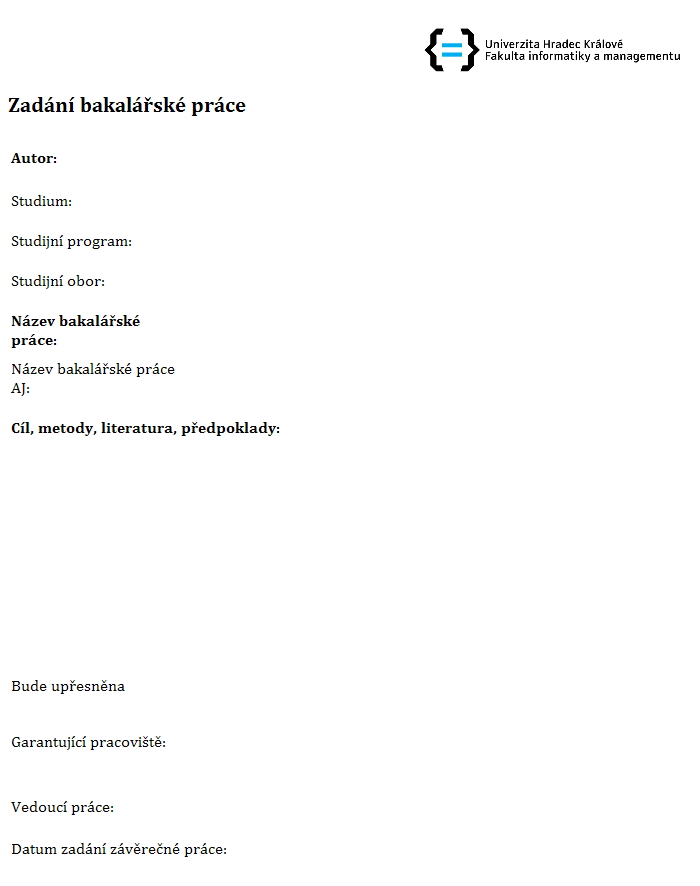
\includepdf[pages=-, offset=20 -50, width=20cm]{images/assignment.png}

\end{document}
